\problemname{Vasaloppet}
\noindent
Charlotte is watching Vasaloppet on TV. The broadcast starts at second $0$ and ends at second $T$.
Unfortunately, there are also $N$ ad breaks, lasting during $N$ non-overlapping intervals of seconds
between second $0$ and second $T$. Charlotte becomes very inspired by seeing the competitors at the starting
line and wants to go skiing herself during the race. The skiing trip takes $S$ seconds, and she must be back by
second $T$ (to see who wins).

Charlotte wants to go on her skiing trip at a time when she misses as little of Vasaloppet as possible.
Your task is to calculate the minimum number of seconds of Vasaloppet that Charlotte can miss if she optimally
chooses when to go on her skiing trip. Missed seconds are the seconds when Charlotte is out on her skiing trip
while there is no ad break running.

\begin{centering}
  \begin{figure}[h]
      \centering
      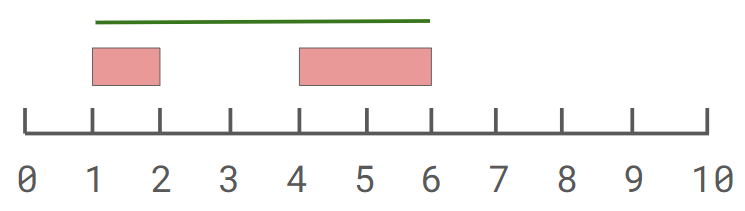
\includegraphics[width=0.6\textwidth]{sample1.PNG}
      \caption{The picture describes the first sample case. The red rectangles are the ad breaks. If Charlotte
      starts her skiing trip when the first ad break starts and gets back home when the second break ends, she only misses
      $2$ seconds of Vasaloppet.}
      \label{fig:enter-label}
  \end{figure}
\end{centering}

\section*{Input}
The first line of input contains three integers $N, T,$ and $S$ ($0 \leq N \leq 10^5$, $1 \leq S \leq T \leq 10^9$). 
$N$ is the number of ad breaks, $T$ is the duration of the broadcast in seconds, and $S$ is the length of the skiing trip in seconds.

The following $N$ lines each contain two integers $l_i, r_i$ ($0 \leq l_i < r_i \leq T$),
indicating that the $i$-th commercial break lasts from second $l_i$ to second $r_i$.\\
The commercial breaks are given in the order they occur, and all breaks are disjoint and sorted, 
which means that $r_i < l_{i+1}$ for $i < N$.

\section*{Output}
Print an integer, the minimum number of seconds that Charlotte can miss of Vasaloppet during her skiing trip if it is
chosen optimally. Note that the skiing trip can end exactly at second $T$. For example, the skiing trip can cover
the entire duration of Vasaloppet if $S=3$ and $T=3$.

\section*{Points}
Your solution will be tested on several test case groups.
To get the points for a group, it must pass all the test cases in the group.

\noindent
\begin{tabular}{| l | l | p{12cm} |}
  \hline
  \textbf{Group} & \textbf{Point value} & \textbf{Constraints} \\ \hline
  $1$    & $10$       & $N=1$ \\ \hline
  $2$    & $25$       & $N \leq 1000$ \\ \hline
  $3$    & $30$       & $T \leq 10^6$ \\ \hline
  $4$    & $35$       & No additional constraints. \\ \hline
\end{tabular}

%\section*{Samples}
